\documentclass[aspectratio=169]{ISAE-Beamer}
\usefonttheme[onlymath]{serif}
\usepackage{amsmath,amssymb,amsthm}
\usepackage{bm}

\usepackage{graphicx}
\usepackage{diffcoeff}
\usepackage{dsfont}
\usepackage{mathrsfs}
\usepackage{tcolorbox}

%\usepackage{multimedia}
\usepackage{media9}
\usepackage[backend=bibtex]{biblatex}

\graphicspath{{../Figures/}}

\bibliography{bib_pres_CDC}

\DeclareMathOperator{\Tr}{Tr}
\DeclareMathOperator*{\grad}{grad}
\DeclareMathOperator*{\Grad}{Grad}
\DeclareMathOperator*{\Div}{Div}
\renewcommand{\div}{\operatorname{div}}
\DeclareMathOperator*{\Hess}{Hess}

\DeclareMathOperator*{\argmax}{arg\,max}
\DeclareMathOperator*{\argmin}{arg\,min}

\def\onedot{$\mathsurround0pt\ldotp$}
\def\cddot{% two dots stacked vertically
	\mathbin{\vcenter{\baselineskip.67ex
			\hbox{\onedot}\hbox{\onedot}}%
}}

\renewcommand\bibfont{\scriptsize}


\makeatletter \renewcommand\d[1]{\ensuremath{%
		\;\mathrm{d}#1\@ifnextchar\d{\!}{}}}
\makeatother

\title[58th CDC conference]{Interconnection of the Kirchhoff plate within the port-Hamiltonian framework}

\institute[ISAE]
{\inst{1}ISAE-SUPAERO, Toulouse}

\author[Andrea Brugnoli]{Andrea Brugnoli\inst{1}, Daniel Alazard\inst{1}, Valérie Pommier-Budinger\inst{1}, Denis Matignon\inst{1}}

\date[Nice, 13/12/19]{December, the 13th, 2019}

%\thanks{}

\begin{document}

\maketitle

\begin{frame}{Outline}

\tableofcontents

\end{frame}

\section{Introduction: discretization of pH Systems}

\begin{frame}{Infinite dimensional pH systems}
\begin{block}{\only<1>{General}\only<2>{Linear} infinite dimensional pH system}
	\begin{equation*}
	\begin{cases}
	\displaystyle \diffp{x}{t}(z, t) &= \mathcal{J} \only<1>{\displaystyle \diffd{H}{x}} \only<2>{\mathcal{Q} x} + B \textcolor{red}{u(z, t)}, \vspace{3pt} \\
	\displaystyle \textcolor{red}{y(z, t)} &= B^* \only<1>{\displaystyle \diffd{H}{x}} \only<2>{\mathcal{Q} x}.
	\end{cases}
	\end{equation*}
	With boundary conditions
	\[\textcolor{blue}{u_\partial} = \mathcal{B} \diffd{H}{x}, \quad \textcolor{blue}{y_\partial} = \mathcal{C} \diffd{H}{x} \]
	Energy rate: $\dot{H} = \displaystyle \textcolor{blue}{u_\partial^T y_\partial} +  \int_{\Omega} \textcolor{red}{u(z, t) y(z, t)} \d{\Omega}$
	\begin{itemize}
		\item $x$ energy variables, $e = \delta_x H = \only<2>{\mathcal{Q} x}$: co-energy variables \only<2>{($\mathcal{Q}$ symmetric positive operator)};
		\item $\mathcal{J}$: skew-symmetric differential operator;
		\item $\mathcal{B}, \mathcal{C}$: boundary operator;
		\item $u, y, B$: distributed input, output and control operator.
	\end{itemize}
\end{block}

\end{frame}


\begin{frame}{Structure preserving discretization}
The main properties of the dpH (conservative, passive system) are preserved at a discrete level.
\begin{columns}[T]
	\setlength{\abovedisplayskip}{1pt}
	\setlength{\belowdisplayskip}{1pt}
	\begin{column}{.4\textwidth}
		\begin{block}{Infinite dimensional pHs \only<2>{(linear case)}}
			PDE:
			\begin{align*}
			\partial_t{x}(z, t) &= \mathcal{J} \only<1>{\displaystyle \diffd{H}{x}} \only<2>{\mathcal{Q} x} + B \textcolor{red}{u(z, t)}, \\
			\textcolor{red}{y(z, t)} &= B^* \delta_x {H}.
			\end{align*}
			Boundary conditions: 
			\[\textcolor{blue}{u_\partial} = \mathcal{B} \only<1>{\displaystyle \diffd{H}{x}} \only<2>{\mathcal{Q} x}, \quad \textcolor{blue}{y_\partial} = \mathcal{C} \only<1>{\displaystyle \diffd{H}{x}} \only<2>{\mathcal{Q} x} \]
			Power balance (Stokes Theorem): 
			\[ \dot{H} = \displaystyle \textcolor{blue}{u_\partial^T y_\partial} +  \int_{\Omega} \textcolor{red}{u(z, t) y(z, t)} \d{\Omega}
			\]
		\end{block}
	\end{column}
	\begin{column}{.4\textwidth}
		\begin{block}{Finite dimensional pHs \only<2>{(linear case)}}
			ODE:
			\begin{align*}
			\dot{x} &= J \only<1>{\displaystyle \partial_x {H}} \only<2>{Q x} + B_d \textcolor{red}{u_d} + B_\partial \textcolor{blue}{u_\partial}, \\
			\textcolor{red}{y_d} &= B_d^T \only<1>{\displaystyle \partial_x {H}} \only<2>{Q x}, \\
			\textcolor{blue}{y_\partial} &= B_\partial^T \only<1>{\displaystyle \partial_x {H}} \only<2>{Q x}
			\end{align*}
			Power balance: 
			\[ \dot{H} = \textcolor{blue}{u_\partial^T y_\partial} +  \textcolor{red}{u_d^T y_d}
			\]
		\end{block}
	\end{column}
\end{columns}

\end{frame}

\begin{frame}{}
\begin{exampleblock}{Available methods}
	\begin{itemize}
		\item Spectral methods (Moulla 2012):
		\begin{itemize}
			\item[\textcolor{green}{\checkmark}] Rapid spectral convergence;
			\item[\textcolor{red}{$\times$}] Only for 1D problem;
		\end{itemize}
		\item Finite differences (Trenchant 2018);
		\begin{itemize}
			\item[\textcolor{green}{\checkmark}] Valid up to 2D geometries;
			\item[\textcolor{red}{$\times$}] Requires \textit{ad hoc} implementation (staggered grids);
		\end{itemize}
		\item Finite elements based
		\begin{itemize}
			\item Golo 2004, Kotyczka 2018: the implementation requires exterior calculus knowledge and depends on the some parameters that ensure the preservation of power flow;		
			\item \textcolor{blue}{Cardoso-Ribeiro 2018}:
			\begin{itemize}
				\item[\textcolor{green}{\checkmark}] Natural extension of the mixed finite element method to pH systems;
				\item[\textcolor{green}{\checkmark}] Implementable using well-established libraries (Fenics, Firedrake);
			\end{itemize}
		\end{itemize}
	\end{itemize}
\end{exampleblock}
\end{frame}

\begin{frame}{Why structure preserving discretization?}
A distributed pH system interconnected to a strictly positive real boundary controller  is asymptotically stable \footfullcite{villegasTAC}. \\
\vspace{1cm}
This allows the construction of observed based controller based on a finite dimensional discretization of the plant \footfullcite{toledo2019observerbased} that guarantees stability of the infinite dimensional system (no spillover effect).

\end{frame}

\section{The Kirchhoff plate as a port-Hamiltonian system}

	
\subsection{Classical formulation}

\begin{frame}{The classical Kirchhoff model}
\only<1>{\begin{block}{Classical bilaplacian formulation}
	For an homogeneous isotropic material
	\begin{equation*}
	\rho h \diffp[2]{w}{t} + D \Delta^2 w = p, \quad \bm{x} \in \Omega \subset \mathbb{R}^2.
	\end{equation*}
	$\Delta^2 = \partial_{xxxx} + 2 \partial_{xxyy} + \partial_{yyyy}$ is the bilaplacian operator
\end{block}}
\only<2>{
\begin{block}{Bending moment formulation}

	\begin{equation*}
	\rho h \diffp[2]{w}{t} + \div\Div(\bm{M}) = p, \quad \bm{x} \in \Omega \subset \mathbb{R}^2.
	\end{equation*}
	Where $\bm{M} = \mathbb{D} \nabla^2 w \in \mathbb{R}^{2\times 2}_{\text{sym}}$ is the bending moment tensor and $\nabla^2 = \Grad \circ \grad$ the Hessian. 
	\[\div\Div(\bm{M}) = \partial_{xx} M_{11} + 2 \partial_{xy} M_{12} + \partial_{yy} M_{22} \]
\end{block}}
\begin{itemize}
	\item $\rho \; [\mathrm{kg/m^3}]$ is the mass density;
	\item $h \; [\mathrm{m}]$ is the plate thickness;
	\item $p \; [\mathrm{N/m^2}]$ is an external distributed force; 
	\only<1>{\item $D \; [\mathrm{Pa \, m}]$ is the bending stiffness;}
	\only<2>{\item $\mathbb{D}$ is the bending rigidity tensor (symmetric, positive). 	For an homogeneous isotropic material
	\begin{equation*}
		\mathbb{D} \bm{A} = D \left\{(1-\nu) \bm{A} + \nu \Tr(\bm{A}) \bm{I}\right\};
	\end{equation*}}
\end{itemize}
\end{frame}

\begin{frame}{Boundary conditions}
\begin{overlayarea}{\textwidth}{\textheight}
For the boundary variables consider the definitions
\begin{equation*}
\begin{aligned}
\text{Flexural moment} \quad M_{nn} &= \bm{M} \cddot (\bm{n}\otimes\bm{n}), \\
\text{Torsional moment} \quad M_{ns} &= \bm{M} \cddot (\bm{n}\otimes\bm{s}),
\end{aligned} \quad
\begin{aligned}
\text{Shear stress} \quad \bm{q} &= \Div \bm{M}, \\
\text{Kirchhoff shear force} \quad \widetilde{q}_n &= - \bm{q}\cdot \bm{n} - \partial_{\bm{s}} M_{ns}.
\end{aligned}
\end{equation*} \\
$\bm{A} \cddot \bm{B} = \sum_{i, j} A_{ij} B_{ij}$ is the tensor contraction and $\bm{a} \otimes \bm{b} = \bm{a} \bm{b}^\top \in \mathbb{R}^{2\times 2}$ is the dyadic product. \\
\begin{tcolorbox}
	\centering
	\only<1>{\large{References} \\ 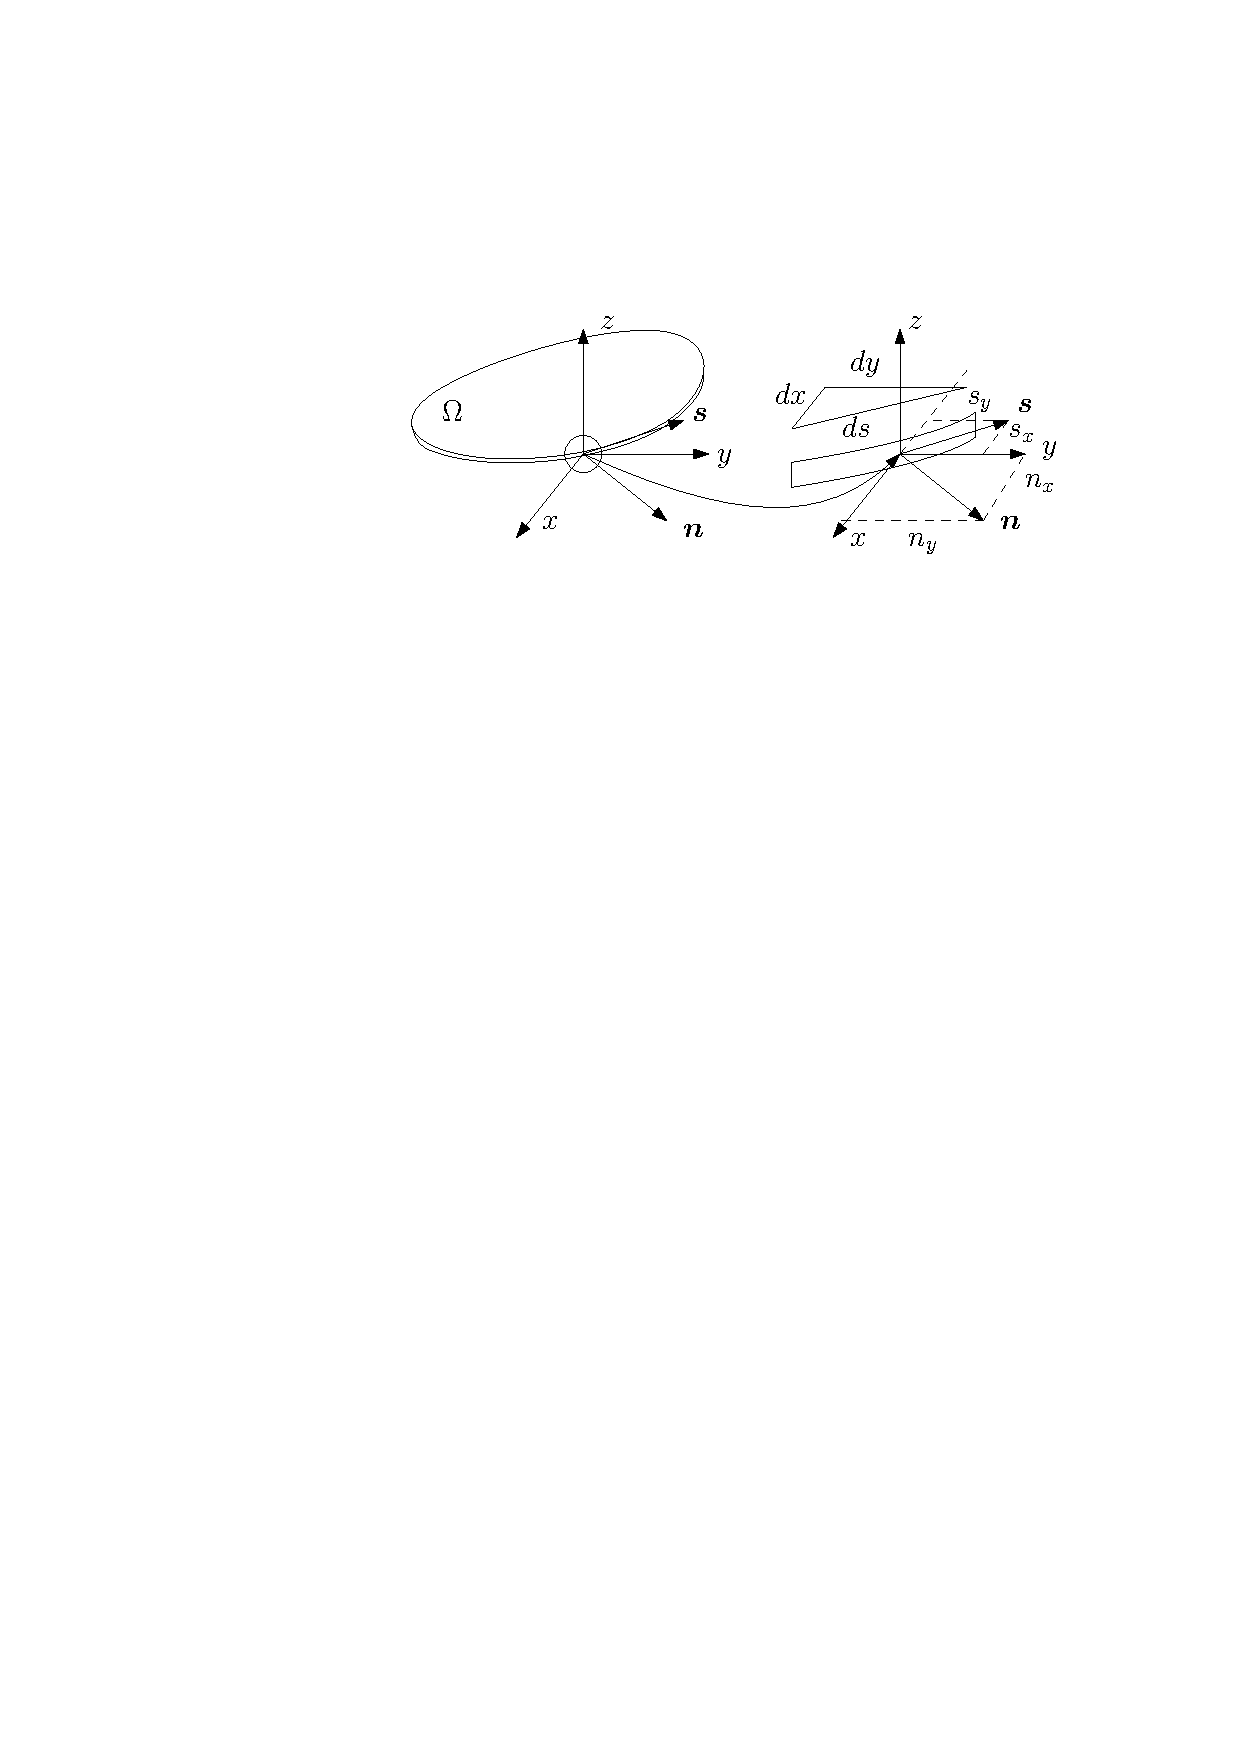
\includegraphics[width=0.7\textwidth]{plate_ref.pdf}}
	\only<2>{\large{Cauchy Law} \\ 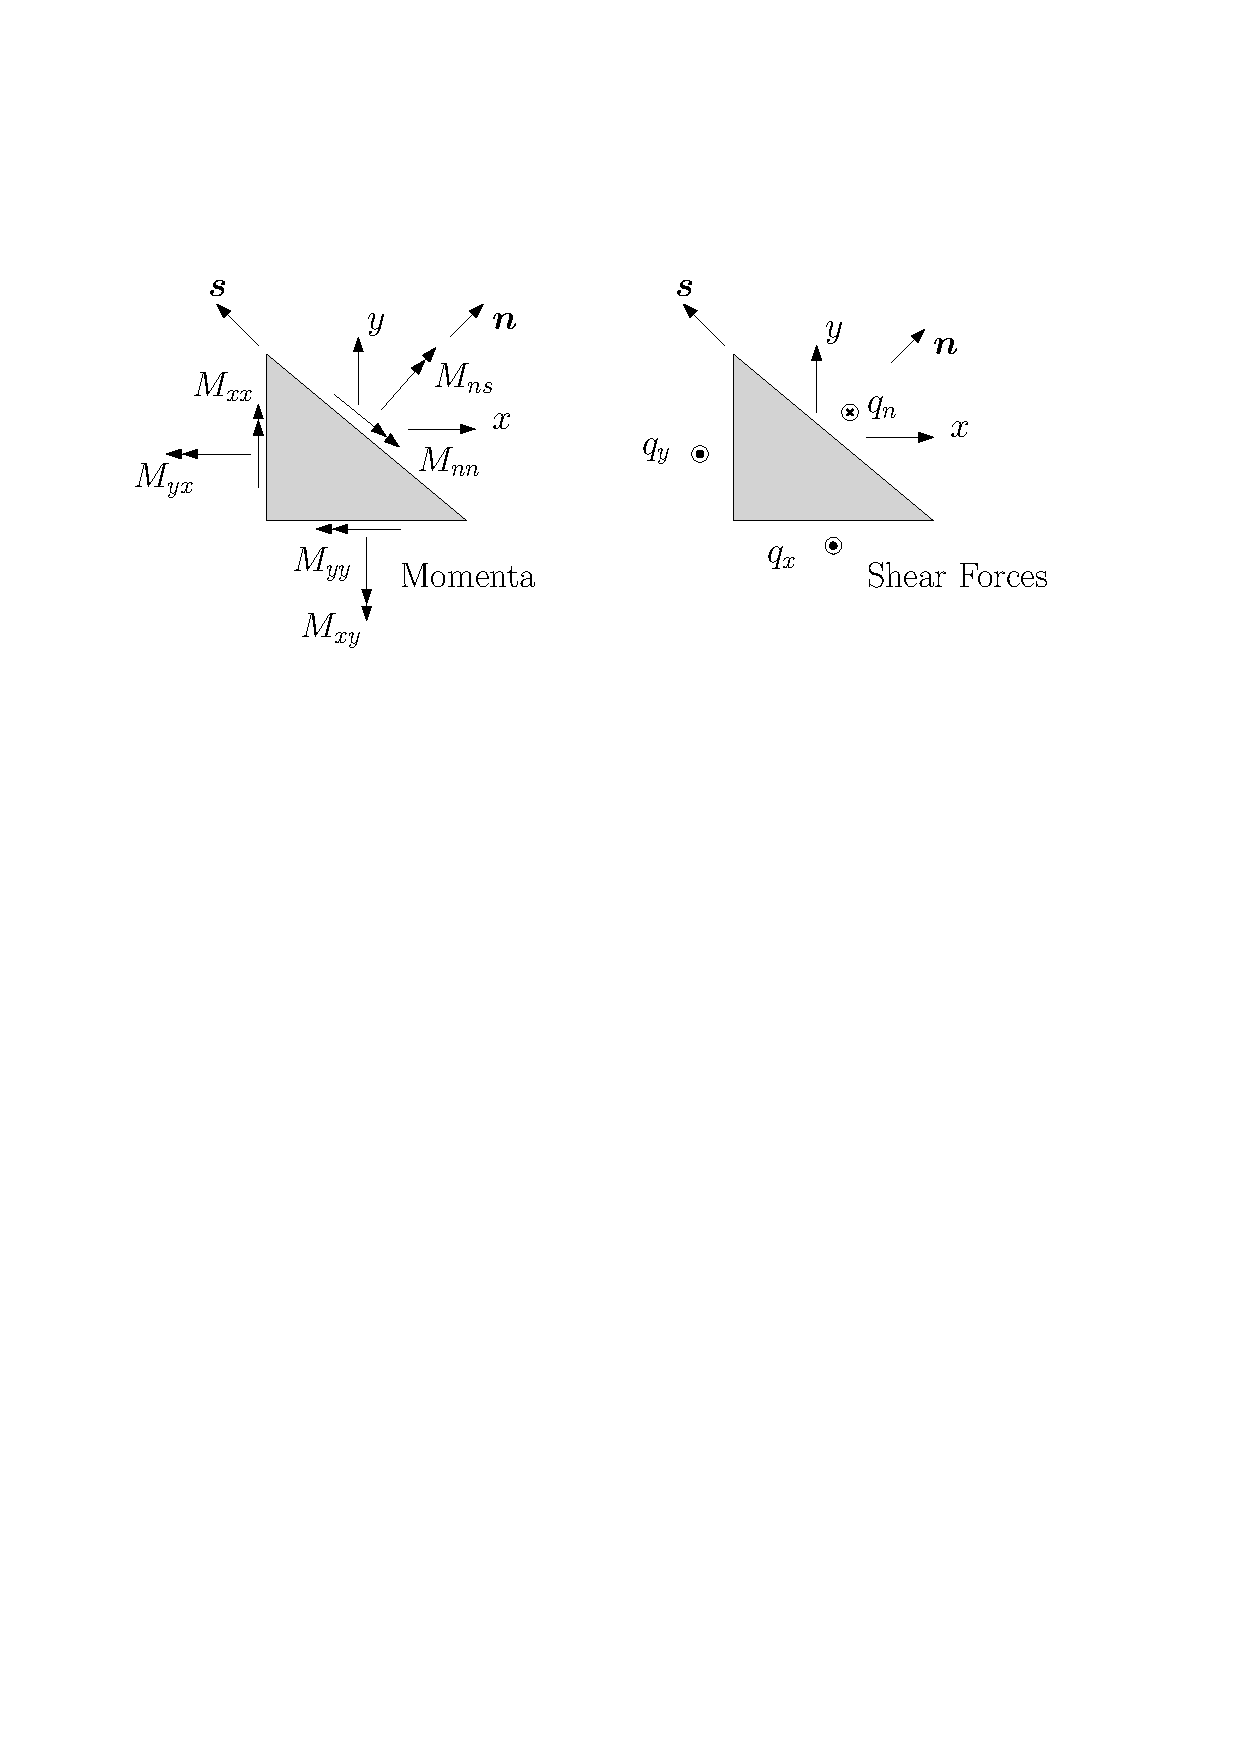
\includegraphics[width=0.6\textwidth]{cauchy_law.pdf}}
	\only<3>{\large{Boundary conditions} \\ 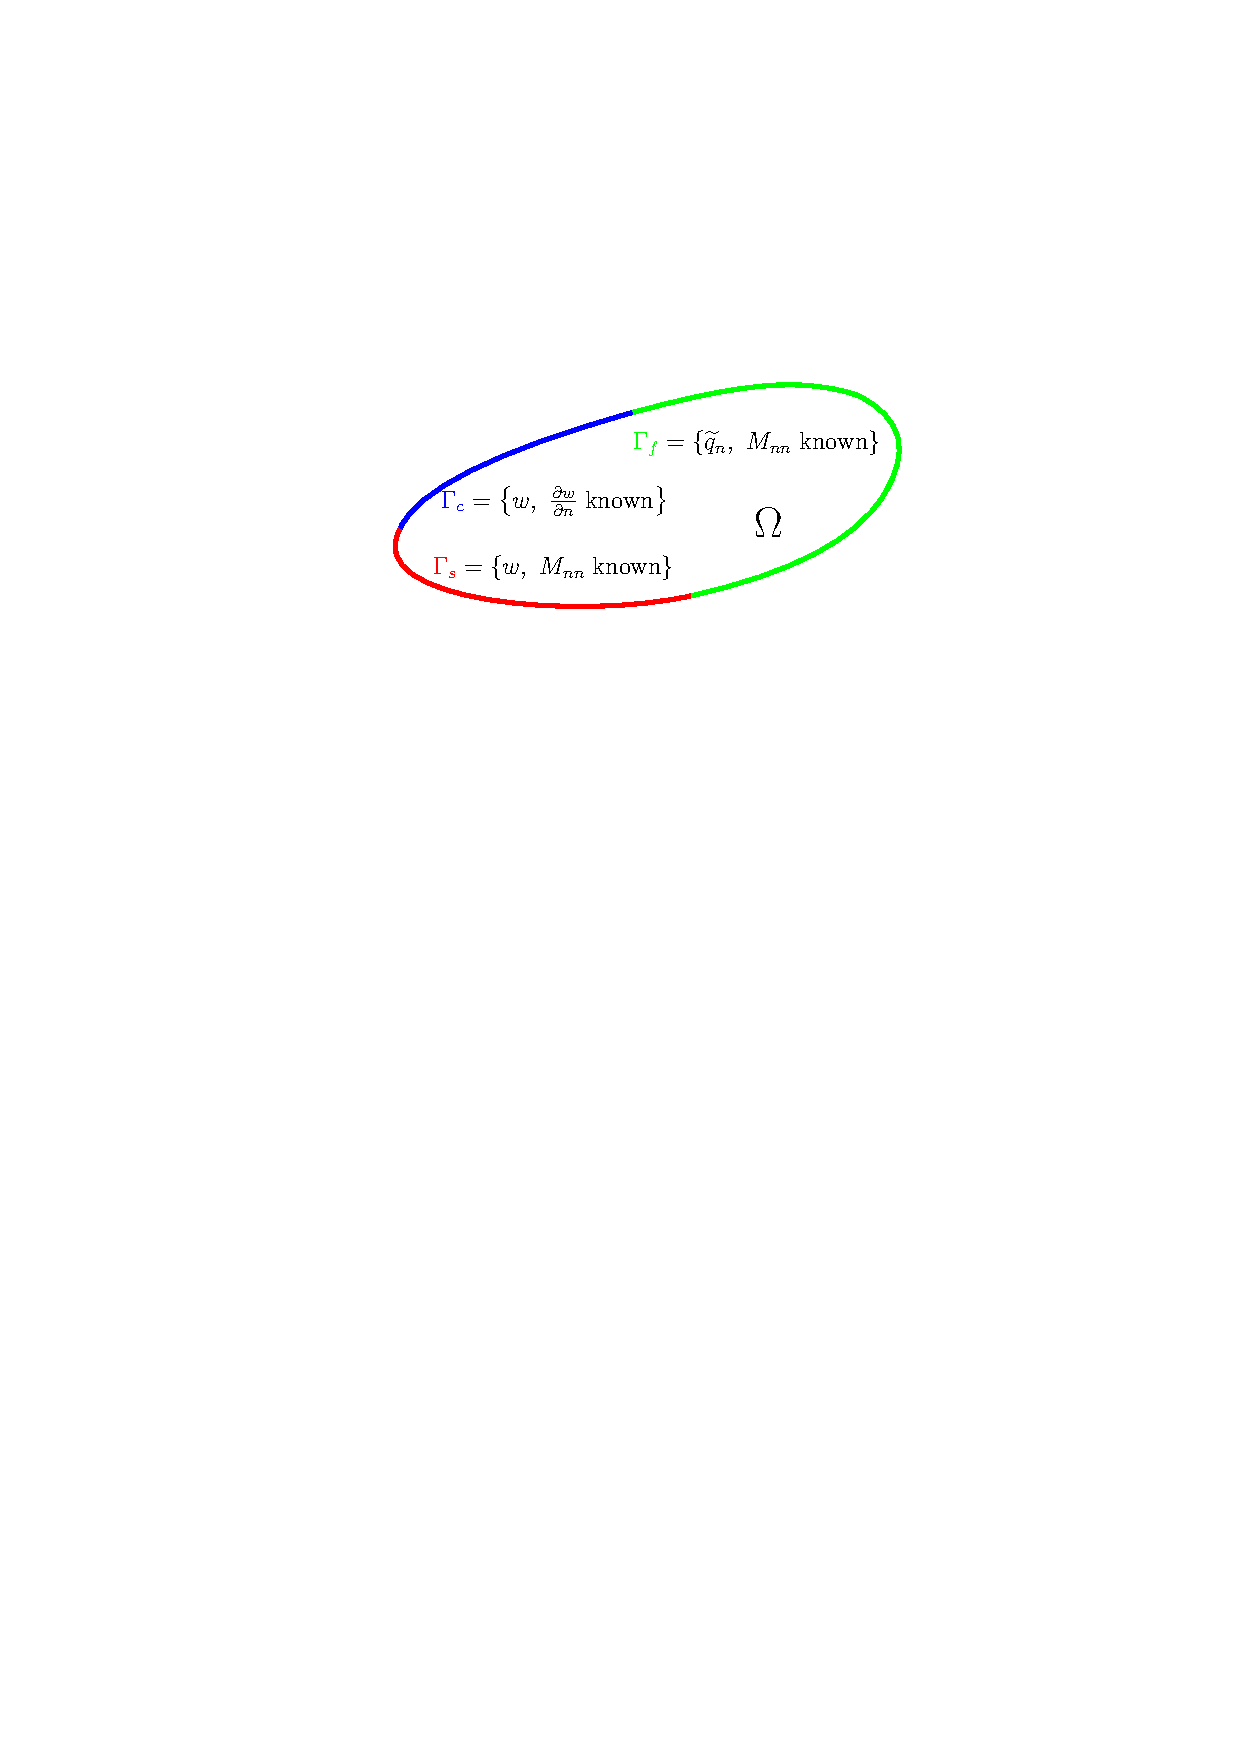
\includegraphics[width=0.6\textwidth]{kirchh_plate_bcs.pdf}}
\end{tcolorbox}
\end{overlayarea}
\end{frame}

\subsection{Port-Hamiltonian formulation}

\begin{frame}{Hamiltonian and energy variables}
The total energy of the system is given by the sum of kinetic and deformation energy
\[
H = \frac{1}{2} \int_{\Omega} \left\{\rho h \left(\partial_t w\right)^2 + \mathbb{D} \nabla^2 w \cddot \nabla^2 w \right\} \d{\Omega}
\] 
Consider the following choice for the energy variables
\begin{align*}
	\alpha_1 &:= \rho h \partial_t w, \quad \text{Linear momentum} \\
	\bm{A}_2 &:=  \nabla^2 w, \quad \text{Curvature}
\end{align*}
This leads to the following co-energy variables
\begin{align*}
e_1 &:= \diffd{H}{\alpha_1} =  \partial_t w, \quad \text{Vertical velocity} \\
\bm{E}_2 &:= \diffd{H}{\bm{A}_2} = \bm{M}, \quad \text{Bending moment}
\end{align*}
\end{frame}

\begin{frame}{Port Hamiltonian formulation}
\begin{tcolorbox}
The system
\begin{equation*}
\diffp{}{t} \begin{pmatrix}
\alpha_1 \\ \bm{A}_2
\end{pmatrix} =
\underbrace{\begin{bmatrix}
0 & -\div\Div \\
\nabla^2 & 0 \\
\end{bmatrix}}_{\mathcal{J}} \begin{pmatrix}
{e}_1 \\ \bm{E}_2
\end{pmatrix}, \quad \begin{pmatrix}
{e}_1 \\ \bm{E}_2
\end{pmatrix} = \underbrace{\begin{bmatrix}
(\rho h)^{-1} & 0 \\
0 & \mathbb{D} \\
\end{bmatrix}}_{\mathcal{Q}}
\begin{pmatrix}
\alpha_1 \\ \bm{A}_2
\end{pmatrix}
\end{equation*}
defines a Stokes-Dirac structure. The proof is readily obtained considering that the following holds
\[ (\div \Div)^* = \nabla^2\]
This means that the operator $\mathcal{J}$ is formally skew-adjoint.
\end{tcolorbox}
It is worth noticing that the boundary variables are defined by the power balance
\[
\dot{H} = \int_{\partial \Omega} \left\{ \textcolor{blue}{\partial_t w} \, \textcolor{red}{\widetilde{q}_n} + \textcolor{blue}{\partial_{\bm{n}} (\partial_t w)} \, \textcolor{red}{M_{nn}} \right\}  \d{s}.
\]

\end{frame}

\section{Structure preserving discretization}

\subsection{The partitioned finite element method}



\begin{frame}{The partitioned finite element method (PFEM)}
General form of a linear pH system in co-energy variables
\begin{equation*}
\mathcal{M} \diffp{e}{t} = \mathcal{J} e, \qquad \mathcal{M} = \mathcal{Q}^{-1}
\end{equation*}

\begin{block}{General procedure for PFEM}
	\setlength{\abovedisplayskip}{1pt}
	\setlength{\belowdisplayskip}{1pt}
	\begin{enumerate}
		\item Put the system into weak form:
		\begin{equation*}
		\left(v, \mathcal{M} \diffp{e}{t} \right)_{\Omega} = \left(v, \mathcal{J} e \right)_{\Omega}.
		\end{equation*}
		\item Apply integration by part on a partition of $\mathcal{J}$:
		\begin{equation*}
		\left(v, \mathcal{J} e \right)_{\Omega} \overbrace{=}^{i.b.p.} j(v, e)_{\Omega} + b(v, u_\partial)_{\partial \Omega},
		\end{equation*}
		so that $j(v, e)_{\Omega}$ is a skew-symmetric bilinear form.
		\item Discretization by Galerkin method (same basis function for test and co-energy variables)
	\end{enumerate}
\end{block}
\end{frame}

\subsection{Application to the Kirchhoff plate}

\begin{frame}{Application to the Kirchhoff plate}
\begin{overlayarea}{\textwidth}{\textheight}
	\vspace{1cm}
Consider the Kirchhoff plate operators
\[
\mathcal{M} = \text{Diag}(\rho h,\; \mathbb{D}^{-1}), \quad 
\mathcal{J} = \begin{pmatrix}
0 & \only<2,4>{\textcolor{red}{-\div\Div}} \only<1,3>{-\div\Div}\\
\only<1,2>{\nabla^2} \only<3,4>{\textcolor{blue}{\nabla^2}} & 0  \\
\end{pmatrix}
\]
\only<2>{Either the \textcolor{red}{first line of the operator $\mathcal{J}$} is integrated by parts
\begin{align*}
	\left(v, \mathcal{J}e \right)_{\Omega} &= \int_{\Omega} \left\{ - v_1 \textcolor{red}{\div\Div} \bm{E}_2 + \bm{V}_2 \cddot \nabla^2 e_1 \right\} \d{\Omega} \\
	&= \underbrace{\int_{\Omega} \left\{ - \nabla^2 v_1 \cddot \bm{E}_2 + \bm{V}_2 \cddot \nabla^2 e_1 \right\} \d{\Omega}}_{j_{\text{Hess}}(\bm{v}, \bm{e})} + \underbrace{\int_{\partial \Omega} \left\{ v_1 \textcolor{red}{q_n} + \partial_{\bm{n}}v_1 \textcolor{red}{M_{nn}} \right\} \d{s}}_{b_N(\bm{v}, \bm{u}_\partial)_{\partial \Omega}}
\end{align*}
}
\only<3>{Either the \textcolor{blue}{second line of the operator $\mathcal{J}$} is integrated by parts
	\begin{align*}
	\left(v, \mathcal{J}e \right)_{\Omega} &= \int_{\Omega} \left\{ - v_1 \div\Div \bm{E}_2 + \bm{V}_2 \cddot \textcolor{blue}{\nabla^2} e_1 \right\} \d{\Omega} \\
	&= \underbrace{\int_{\Omega} \left\{ - v_1 \div\Div \bm{E}_2 + \div\Div \bm{V}_2 \; e_1 \right\} \d{\Omega}}_{j_{\div\Div}(\bm{v}, \bm{e})} + \underbrace{\int_{\partial \Omega} \left\{ v_{q_n} \textcolor{blue}{\partial_t w} + v_{m_{n}} \textcolor{blue}{\partial_{\bm{n}} \partial_t w} \right\} \d{s}}_{b_D(\bm{v}, \bm{u}_\partial)_{\partial \Omega}},
	\end{align*}
	where $v_{q_n} = - (\Div \bm{V}_2) \cdot \bm{n} - \partial_{\bm{s}} v_{m_s}, \;  v_{m_s} = \bm{V}_2 \cddot (\bm{n} \otimes \bm{s}), \; v_{m_n} = \bm{V}_2 \cddot (\bm{n} \otimes \bm{n})$
}
\only<4>{
	\center
	The selection depends on the control variables. For \textcolor{red}{Neumann} control the first line is integrated by parts. For \textcolor{blue}{Dirichlet control} the second.}
\end{overlayarea}
\end{frame}

\begin{frame}{Finite element choice}
\begin{overlayarea}{\textwidth}{\textheight}
Selecting as control variables the forces and torques (Neumann boundary conditions), the following weak form is obtained:
\[ m(\bm{v}, \partial_t \bm{e}) = j_{\text{Hess}}(\bm{v}, \bm{e}) + b_N(\bm{v}, \bm{u}_\partial)_{\partial \Omega}.
\]
For both $\bm{e}_1, \bm{E}_2$ the $H^2$ conforming Bell elements are selected.  Dirichlet boundary conditions are enforced by Lagrange multipliers, i.e. $\bm{u}_\partial\vert_{\Gamma_D} = \bm{\lambda}$. Those are discretized using quadratic Lagrange polynomials.
\only<1>{
	\begin{tcolorbox}
	\centering
	\includegraphics[width=0.5\textwidth]{elements.eps}
	\end{tcolorbox}
}
\only<2>{

\begin{equation*}
\begin{aligned}
\begin{bmatrix}
{M} & {0} \\
{0} & {0} \\
\end{bmatrix}\frac{d}{d t}
\begin{pmatrix}
\bm{e}\\
\bm{\lambda} \\
\end{pmatrix}
&= \begin{bmatrix}
{J} & {G} \\
-{G}^T & {0} \\
\end{bmatrix}
\begin{pmatrix}
\bm{e} \\
\bm{\lambda} \\
\end{pmatrix} + \begin{bmatrix}
{B} \\
0 \\
\end{bmatrix} \bm{u}, \\
{y} &= \begin{bmatrix}
{B}^T & {0} \\
\end{bmatrix} \begin{pmatrix}
\bm{e}\\
\bm{\lambda} \\
\end{pmatrix},
\end{aligned} 
\end{equation*}
}
\end{overlayarea}
\end{frame}



\section{Interconnection with rigid elements}

\begin{frame}{Rigid rod welded to a cantilever plate }
\begin{tcolorbox}
	\centering
	\only<1>{ 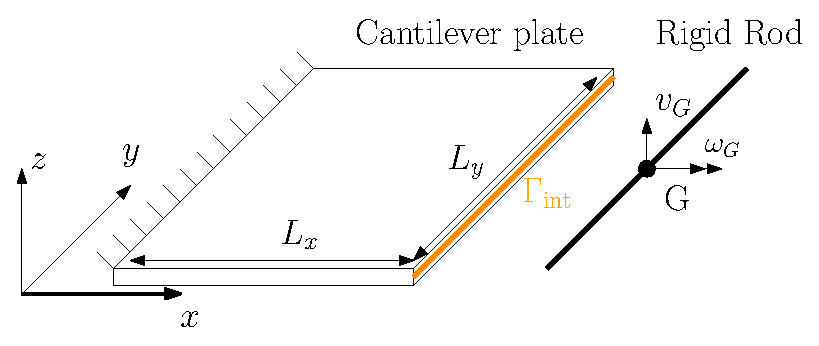
\includegraphics[width=0.9\textwidth]{plate_rod_separated.eps}}
	\only<2>{ \includegraphics[width=0.7\textwidth]{plate_rod_welded.eps}}
\end{tcolorbox}

\end{frame}

\begin{frame}{Boundary interconnection of the Kirchhoff plate}
The system is composed by a cantilever plate (distributed pH) connected to a rigid rod
\only<1>{
\begin{equation*}
\small \text{dpH} \left\{ 
\begin{aligned}
\diffp{x_1}{t} &= \mathcal{J} \diffd{H_1}{x_1} \\
u_{\partial, 1}  &= \mathcal{B} \diffd{H_1}{x_1} \\
y_{\partial, 1} &= \mathcal{C} \diffd{H_1}{x_1} 
\end{aligned}
\right. \qquad
\text{pH} \left\{ 
\begin{aligned}
\diff{\bm{x}_2}{t} &= {J} \diffp{H_2}{\bm{x}_2} + {B} \bm{u}_2 \\
\bm{y}_{2} &= {B}^T \diffp{H_2}{{x}_2} + {D} \bm{u}_2 \\
\end{aligned}, \qquad 
\right. 
\end{equation*} %

where $u_{\partial, 1}  \in \mathscr{U}, \, y_{\partial, 1} \in  \mathscr{Y} = \mathscr{U}^\prime$ belong to some Hilbert spaces and ${x}_2 \in \mathbb{R}^n, {u}, {y} \in \mathbb{R}^m$. The interconnection is power-preserving if
\[
\left\langle u_{\partial, 1}, \; y_{\partial, 1} \right\rangle_{\mathscr{U} \times \mathscr{Y}} + 
\left\langle {u}_{2}, \; {y}_{2} \right\rangle_{\mathbb{R}^m} = 0.
\]
This is achieved by introducing a compact operator $\mathcal{W}: \mathscr{Y} \rightarrow \mathbb{R}^m$
\begin{equation*}
\label{eq:int_inf}
{u}_2 = -\mathcal{W} \, y_{\partial, 1},  \qquad u_{\partial, 1} = \mathcal{W}^* \, {y}_2,
\end{equation*}
}
	
\only<2>{\vspace{.5cm}\centering 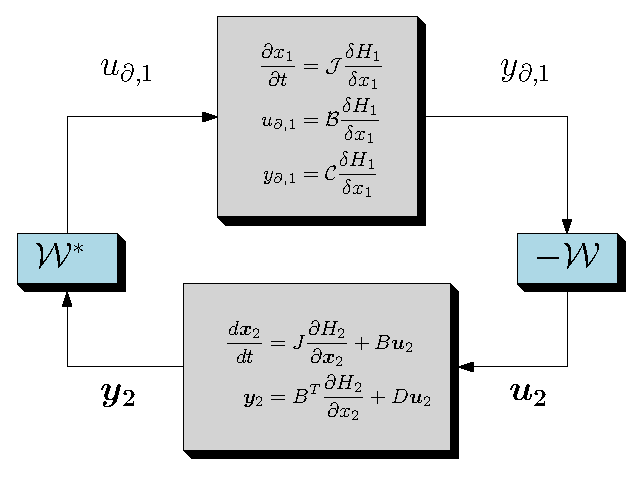
\includegraphics[width=0.6\textwidth]{pp_interconnection.eps}}

\end{frame}

\begin{frame}{Boundary interconnection of the Kirchhoff plate}
\begin{equation*}\small
\begin{aligned}
\text{Plate} \; (\Omega &= [0, L_x] \times [0, L_y]) \\
\begin{bmatrix}
\rho h & 0 \\ 0 & \mathbb{D}^{-1} \\
\end{bmatrix}
\diffp{}{t}
\begin{bmatrix}
\partial_t w \\ \bm{M} \\
\end{bmatrix} &= 
\begin{bmatrix}
0 & -\div\Div \\ \nabla^2 & 0 \\
\end{bmatrix}
\begin{bmatrix}
\partial_t w \\ \bm{M} \\
\end{bmatrix} \\
u_{\partial, \text{pl}} &= \partial_t w (x = L_x, y), \\
y_{\partial, \text{pl}} &= \widetilde{q}_n(x = L_x, y).
\end{aligned} \qquad \quad
\begin{aligned}
\text{Rigid rod} \\
\begin{bmatrix}
M & 0 \\
0   & J_G \\
\end{bmatrix} 
\displaystyle \diff{}{t}
\begin{pmatrix}
v_G \\ \omega_G \\
\end{pmatrix} & = \begin{pmatrix}
F_z \\ T_x \\
\end{pmatrix} = \bm{u}_{\text{rod}}\vspace{1mm}, \\
\bm{y}_{\text{rod}} &= \begin{pmatrix}
v_G \\ \omega_{G} \\
\end{pmatrix},
\end{aligned}
\end{equation*}
Space $\mathscr{Y}$ is the space of square-integrable functions with support on $\Gamma_{\text{int}} = \left\{ (x,y) \vert \; x=L_x, 0 \le y \le L_y  \right\}$.
 The interconnection operator then provides the total force and torque acting on the rigid rod
\begin{equation*}
\mathcal{W} y_{\partial, \text{pl}} =  - \begin{pmatrix}
F_z \\
T_x \\
\end{pmatrix} = \begin{pmatrix}
\int_{\Gamma_{\text{int}}} y_{\partial, \text{pl}} \d{s} \\
\int_{\Gamma_{\text{int}}} \left( y - L_y/2 \right) y_{\partial, \text{pl}} \d{s} \\
\end{pmatrix}.
\end{equation*}
The adjoint operator provides a rigid movement as the plate input at $\Gamma_{\text{int}}$
\begin{align*}
\left\langle \mathcal{W} y_{\partial, \text{pl}}, \; \bm{y}_{\text{rod}} \right\rangle_{\mathbb{R}^m} &= \left\langle y_{\partial, \text{pl}}, \, \mathcal{W}^* \bm{y}_{\text{rod}}\right\rangle_{L^2(\Gamma_{\text{int}})}, \\
\mathcal{W}^* {y}_{\text{rod}} &= v_G + \omega_{G} \left( y - L_y/2 \right).
\end{align*}
\end{frame}

\begin{frame}{Results}
\begin{center}
	\onslide*<1>{
		\setlength{\abovedisplayskip}{0pt}
		\setlength{\belowdisplayskip}{0pt}
		Distributed load ($t_{\text{end}} = 10 \, [\mathrm{ms}]$)
		\begin{equation*}
		p = \begin{cases}
		10^5 \left[ y + 10 \left( y - L_y/2 \right)^2 \right] [Pa], \quad &\forall \, t < 2 \, [\mathrm{ms}], \\
		0, \quad &\forall \, t \ge 2 \, [\mathrm{ms}].
		\end{cases}
		\end{equation*}
		\begin{columns}
			\begin{column}{.45\textwidth}
				\includemedia[
				label=vidNoRod,
				addresource=../Videos/Kirchh_NoRod_Slow.mp4,
				activate=pageopen,
				width=6cm, height=5cm,
				flashvars={
					source=../Videos/Kirchh_NoRod_Slow.mp4
					&loop=true
				}
				]{}{VPlayer.swf}
			\end{column}
			\begin{column}{.45\textwidth}
				\includemedia[
				label=vidRod,
				addresource=../Videos/Kirchh_Rod_Slow.mp4,
				activate=pageopen,
				width=6cm, height=5cm,
				flashvars={
					source=../Videos/Kirchh_Rod_Slow.mp4
					&loop=true
				}
				]{}{VPlayer.swf}
			\end{column}
		\end{columns}
	
	\mediabutton[
	mediacommand=vidNoRod:playPause,
	mediacommand=vidRod:playPause
	]{\fbox{Play/Pause}}
				
		%\movie[width=0.8\textwidth, height=0.6\textheight]{Plate and rod}{../Videos/Comparison_RodNoRod.mp4}	
	}
		\onslide*<2>{
			\includegraphics[width=0.48\textwidth]{InterconnectionRod/HamiltonianNoRod_cropped.eps}
			\includegraphics[width=0.48\textwidth]{InterconnectionRod/HamiltonianRod_cropped.eps}
		}
	\end{center}
\end{frame}

\section{Stabilization by boundary injection}

\begin{frame}{Boundary control of a cantilever plate}
\begin{tcolorbox}
	\centering
	Cantilever plate at the left side and controlled elsewhere
	\includegraphics[width=0.9\textwidth]{plate_controlled.eps}

\end{tcolorbox}
\end{frame}

\begin{frame}{Boundary stabilization of the Kirchhoff plate}
\only<1>{Consider the problem
	\begin{equation*}\small
	\begin{bmatrix}
	\rho h & 0 \\ 0 & \mathbb{D}^{-1} \\
	\end{bmatrix}
	\diffp{}{t}
	\begin{bmatrix}
	\partial_t w \\ \bm{M} \\
	\end{bmatrix} = 
	\begin{bmatrix}
	0 & -\div\Div \\ \nabla^2 & 0 \\
	\end{bmatrix}
	\begin{bmatrix}
	\partial_t w \\ \bm{M} \\
	\end{bmatrix} \quad (x, y) \in \Omega = [0, 1]\times[0,1]
	\end{equation*}
	subjected to the following boundary conditions
	\begin{align*}
	\begin{aligned}
	\partial_t w|\textcolor{blue}{\Gamma_D} &= 0, \\
	\partial_x \partial_t w|\textcolor{blue}{\Gamma_D} &= 0, \\
	\end{aligned} \qquad \textcolor{blue}{\Gamma_D} &= \left\{x = 0 \right\}\\
	\begin{aligned}
	{M}_{nn}|\textcolor{red}{\Gamma_N} &= u_M, \; \\
	\widetilde{q}|\textcolor{red}{\Gamma_N} &= u_F,\\
	\end{aligned} \qquad \textcolor{red}{\Gamma_N} &= \left\{y = 0 \cup x=1 \cup y=1 \right\}
	\end{align*}
	
	with initial conditions (compatible with the constraints):
	\[
	\partial_t w(x,y,0) = x^2; \qquad \bm{M}(x,y,0) ={0}.
	\]
}
\only<2>{ Obtain a finite-dimensional uncontrolled system
	\begin{equation*}
	\begin{aligned}
	\begin{bmatrix}
	{M} & {0} \\
	{0} & {0} \\
	\end{bmatrix}\frac{d}{d t}
	\begin{pmatrix}
	\bm{e}\\
	\bm{\lambda} \\
	\end{pmatrix}
	&= \begin{bmatrix}
	{J} & {G} \\
	-{G}^T & {0} \\
	\end{bmatrix}
	\begin{pmatrix}
	\bm{e} \\
	\bm{\lambda} \\
	\end{pmatrix} + \begin{bmatrix}
	{B} \\
	0 \\
	\end{bmatrix} \bm{u}, \\
	{y} &= \begin{bmatrix}
	{B}^T & {0} \\
	\end{bmatrix} \begin{pmatrix}
	\bm{e}\\
	\bm{\lambda} \\
	\end{pmatrix},
	\end{aligned} 
	\end{equation*}
	Apply the control law $\bm{u} = -K\bm{y}, \ K>0$
	\begin{equation*}
	\begin{bmatrix}
	M & {0} \\
	{0} & {0} \\
	\end{bmatrix}
	\frac{d}{d t}
	\begin{pmatrix}
	\bm{e}\\
	\bm{\lambda} \\
	\end{pmatrix}
	= \begin{bmatrix}
	{J} - {R} & {G} \\
	-{G}^T & {0} \\
	\end{bmatrix}
	\begin{pmatrix}
	\bm{e}\\
	\bm{\lambda} \\
	\end{pmatrix},
	\end{equation*}
	with ${R} = {B} {K} {B}^T \succeq 0$. \\
	The Hamiltonian $\dot{H} = - \bm{e}^T R \bm{e} \le 0$ is a non increasing function and by La~Salle principle the equilibrium point $\bm{e} = 0$ is asymptotically stable.	
}

\end{frame}
\begin{frame}
\begin{center}
	\only<1>{Control parameter ($t_{\text{end}} = 5 [\mathrm{s}]$)
		\begin{equation*}
		K = 
		\begin{cases}
		0, \quad &\forall t < 1 \, [\mathrm{s}], \\
		100, \quad &\forall t \ge 1 \, [\mathrm{s}].
		\end{cases}
		\end{equation*}
		\vspace{.1cm} \\
		\includemedia[
		label=vidDam,
		addresource=../Videos/Kirchh_Damped_4faster.mp4,
		activate=pageopen,
		width=10cm, height=5cm,
		flashvars={
			source=../Videos/Kirchh_Damped_4faster.mp4
			&loop=true
		}
		]{}{VPlayer.swf}
		
		\mediabutton[
		mediacommand=vidDam:playPause,
		]{\fbox{Play/Pause}}
		
		%\movie[width=0.42\textwidth, height = 0.7 \textheight]{Damped Kirchhoff Plate}{../Videos/Kirchh_Damped_4faster.mp4}			
	}
	\only<2>{
		\includegraphics[height=0.9\textheight]{DampingInjection/HamiltonianDamped_cropped.eps}
	}
\end{center}
\end{frame}

\begin{frame}{Conclusion}
The following has been presented:
	\begin{itemize}
	\onslide<2->{\item the Kirchhoff plate model as a port Hamiltonian system;}
	\onslide<3->{\item a structure preserving discretization method capable of dealing with generic bcs;}
	\onslide<4->{\item interconnection with rigid elements (multibody framework);}
		\onslide<5->{\item a simple control application by damping injection;}
	\end{itemize}
	\onslide<6->{Still no rigorous proof of convergence for the finite elements. Existing solutions (only for static problems):}
	\begin{itemize}
		\onslide<7->{\item The Hellan-Herrmann-Johnson  method \footfullcite{Blum1990}, but difficulties when dealing with inhomogeneous bcs;}
		\onslide<8->{\item New discretization method capable that handles inhomogeneous bcs \footfullcite{RafetsederSIAM}.}
	\end{itemize}
\end{frame}


\begin{frame}{}
\centering
\Huge Thanks for your attention \\
\Huge Questions?
\end{frame}

\begin{frame}[allowframebreaks]{References}
\printbibliography
\nocite{*}
\end{frame}

\end{document}
